
\documentclass[10pt,a4paper,twocolumn]{article}
\usepackage[a4paper,top=0.75in,bottom=0.75in,left=0.7in,right=0.7in,columnsep=0.28in]{geometry}
\usepackage[T1]{fontenc}
\usepackage[utf8]{inputenc}
\usepackage{lmodern}
\usepackage{microtype}
\usepackage{amsmath,amssymb}
\usepackage{graphicx}
\usepackage{xcolor}
\usepackage{booktabs}
\usepackage{array}
\usepackage{float}
\usepackage{enumitem}
\usepackage{caption}
\usepackage{xurl}
\usepackage{placeins}
\usepackage{balance}
\usepackage{stfloats}
\usepackage{pgfplots}
\pgfplotsset{compat=1.18, every axis/.append style={font=\small}}
\usetikzlibrary{positioning, arrows.meta}
\usepackage{fancyhdr}
\usepackage{authblk}
\usepackage{cite}
\usepackage{titlesec}
\usepackage{lettrine}
\usepackage[most]{tcolorbox}
\usepackage{hyperref}
\hypersetup{colorlinks=false,hidelinks}

% Colors
\definecolor{radblue}{RGB}{0,73,144}

% Section formatting
\titleformat{\section}{\large\bfseries\color{radblue}}{\thesection}{0.8em}{}
\titleformat{\subsection}{\normalsize\bfseries\color{radblue}}{\thesubsection}{0.8em}{}
\titleformat{\subsubsection}{\normalsize\itshape\bfseries}{\thesubsubsection}{0.8em}{}
\titlespacing{\section}{0pt}{1.0ex plus 0.5ex}{0.3ex}
\titlespacing{\subsection}{0pt}{0.8ex plus 0.3ex}{0.2ex}
\titlespacing{\subsubsection}{0pt}{0.5ex plus 0.2ex}{0.1ex}

% Float placement parameters for twocolumn mode
\setcounter{dbltopnumber}{4}
\renewcommand{\dbltopfraction}{0.92}
\renewcommand{\dblfloatpagefraction}{0.85}
\renewcommand{\textfraction}{0.07}

% Table/caption settings
\setlength{\tabcolsep}{4pt}
\renewcommand{\arraystretch}{1.15}
\emergencystretch=3em
\captionsetup{font=small,labelfont=bf}

% Running headers
\pagestyle{fancy}
\fancyhf{}
\fancyhead[L]{\small\textit{Multi-View Fusion for Breast Cancer Detection on VinDr-Mammo}}
\fancyhead[R]{\small\thepage}
\renewcommand{\headrulewidth}{0.4pt}

% Paragraph style
\setlength{\parindent}{1.5em}
\setlength{\parskip}{0.2em plus 0.1em}

% Custom commands
\newcommand{\auc}{\mathrm{AUROC}}
\newcommand{\satninety}{S@90\%spec}
\newcommand{\vindr}{VinDr-Mammo}
\newcommand{\rsna}{RSNA 2022}
\newcommand{\mamnet}{MamNet-6}

\title{\textbf{\mamnet{}: Multi-View Fusion, CrossView Transformer, and Uncertainty-Aware Triage for Breast Cancer Detection on \vindr}}
\author[1]{Haoming Luo}
\author[1]{Matthew Hamilton}
\author[1]{Oscar Meruvia-Pastor}
\author[1]{Edward Kendall}
\affil[1]{\small Department of Computer Science, Memorial University, St.\ John's, NL, Canada}
\date{May 20, 2026}

\begin{document}
\twocolumn[{%
\maketitle
\vspace{-0.5em}
\begin{tcolorbox}[
  colback=gray!7, colframe=radblue,
  arc=2pt, boxrule=0.5pt,
  left=5pt, right=5pt, top=5pt, bottom=5pt,
  before upper={\small},
]
\textbf{Background:} Breast cancer is the most commonly diagnosed cancer worldwide. Population screening based on full-field digital mammography (FFDM) reduces mortality but imposes heavy radiologist workload and substantial inter-reader variability, motivating computer-aided diagnosis.

\smallskip
\textbf{Purpose:} To develop and evaluate \mamnet{}, a six-stage pipeline for breast cancer detection on the \vindr{} FFDM benchmark from Vietnam, progressing from single-view CNN baselines to a multi-view ensemble with uncertainty-aware triage simulation.

\smallskip
\textbf{Materials and Methods:} We trained five single-view CNN backbones (Stage~1), a shared-backbone BreastPairNet multi-view network across twelve backbone$\times$fusion$\times$resolution variants (Stage~2), a CrossView Transformer with spatial cross-attention (Stage~3), and a bounding-box annotation ablation study (Stage~3b). We then applied Monte Carlo (MC) Dropout for uncertainty quantification (Stage~4), assembled a 16-model ensemble with test-time augmentation (TTA) (Stage~5), and evaluated a Verboom-style hybrid triage simulation (Stage~6). External zero-shot validation was performed on the \rsna{} dataset.

\smallskip
\textbf{Results:} DenseNet-121 attained AUROC=0.7564 (Stage~1). BreastPairNet improved to AUROC=0.8256 [95\,\% CI 0.776--0.871] (+9.1\%, Stage~2); CrossView Transformer reached AUROC=0.8317 [0.783--0.875] (+10.0\%, Stage~3). Adjacent-stage differences lie within overlapping confidence intervals; the ensemble's cumulative gain over Stage~1 is the most statistically robust comparison. Bounding-box annotations degraded AUROC by 0.12--0.20. The 16-model ensemble achieved AUROC=0.8458 (+11.8\% vs Stage~1) with S@90\%spec=0.6566 and PPV=0.184 at the triage threshold. Hybrid triage at 50\% AI reads preserved 87.9\% sensitivity under oracle conditions. External \rsna{} AUROC=0.6008.

\smallskip
\textbf{Conclusion:} A six-stage multi-view pipeline achieves AUROC=0.8458 (PPV=0.184) on \vindr{}. Stage-to-stage AUROC gains are consistent but individually within bootstrap sampling noise; the pipeline's value lies in its cumulative 11.8\% improvement over single-view CNN and in the negative findings. Bounding-box shortcut learning is a key negative finding; domain generalisation to the \rsna{} dataset remains an open challenge.
\end{tcolorbox}
\smallskip
\noindent\textbf{Keywords:} breast cancer detection; mammography; \mamnet{}; multi-view learning; uncertainty quantification; triage; \vindr{}.
\vspace{1.2em}
}]

\section*{Key Results at a Glance}

\begin{table*}[tbp]
\centering
\caption{Summary of the main AUROC results across the six-stage pipeline.}
\label{tab:key-results}
\begin{tabular}{@{}p{0.13\textwidth} p{0.42\textwidth} p{0.10\textwidth} p{0.22\textwidth}@{}}
\toprule
Stage & Method & AUROC & vs.\ single-view \\
\midrule
Prior work & MamT4 \cite{18} (4-view Transformer)\(\ddagger\) & 0.840 & --- \\
Stage 1 & DenseNet-121 (best single-view) & 0.756 & baseline \\
Stage 2 & EfficientNet-B3 +reg (BreastPairNet) & 0.826 & \textbf{+9.1\%} \\
Stage 3 & ConvNeXt-Base (CrossView Transformer) & 0.832 & \textbf{+10.0\%} \\
Stage 4 & DenseNet-121/concat MC Dropout & 0.810 & sensitivity \(\uparrow\) \\
\textbf{Stage 5} & \textbf{16-model ensemble + TTA\(\times\)5} & \textbf{0.846} & \textbf{+11.8\% \(\star\)} \\
External & \rsna{} (zero-shot transfer) & 0.601 & domain gap \textbf{!} \\
\bottomrule
\end{tabular}
\end{table*}

Sensitivity at 90\% specificity (\satninety{}) on \vindr{}: \textbf{0.6566} (best ensemble) vs 0.1636 (\rsna{}). The results suggest that the conservative end of the decision surface is most affected by domain shift, which may be due to a large domain gap between the Vietnamese \vindr{} training data and the \rsna{} screening population.

\section{Introduction}

\lettrine[lines=2, lraise=0.1]{B}{reast} cancer is the most commonly diagnosed cancer worldwide and a leading cause of cancer-related death in women \cite{4}. Population screening programmes based on full-field digital mammography (FFDM) have repeatedly been shown to reduce breast-cancer mortality, yet they impose a heavy operational burden: in many countries each screening exam is double-read by two radiologists, and reader sensitivity varies by 10--30 percentage points between individuals \cite{10,11}. False-negative rates of 10--30\% and false-positive recall rates of approximately 8\% are well documented across both clinical practice and large computer-aided diagnosis literature, with historical hand-engineered detection systems failing to deliver measurable benefit in routine screening \cite{17}.

Deep learning has dramatically improved the situation. CNNs trained on hundreds of thousands of exams now reach or exceed individual radiologist AUC on internal and some external cohorts \cite{11}, and meta-analyses report pooled AUC of 0.87 for AI on digital mammography versus 0.81 for radiologists \cite{4}. Three trends are particularly relevant. First, multi-view modelling that fuses the craniocaudal (CC) and mediolateral oblique (MLO) projections improves over single-view inference because findings often appear unambiguously in only one view \cite{10}. Second, transformer-based fusion of views allows feature-level interaction rather than score-level averaging. Third, uncertainty-aware inference via Monte Carlo (MC) Dropout \cite{13} enables a \emph{hybrid triage} protocol in which the AI reads the most-confident exams autonomously and refers the rest to a human reader \cite{12}, reducing radiologist workload by approximately 38\% in retrospective evaluation \cite{12}.

The \vindr{} benchmark \cite{1} is a 20,000-image, patient-level, 4-view FFDM dataset. Three gaps in the literature are evident. \textbf{(i) Single-view dominance.} Most published \vindr{} results train one image at a time. \textbf{(ii) Spatial cross-view attention is underexplored.} Existing multi-view designs typically concatenate global features. \textbf{(iii) Uncertainty quantification and triage simulation are rare.} No published study has applied MC Dropout to \vindr{} and simulated a Verboom-style triage policy \cite{12}.

This paper makes seven contributions. First, we present a systematic comparison of five single-view CNN backbones. Second, we introduce \textbf{BreastPairNet}, a shared-backbone multi-view network evaluated across twelve backbone$\times$fusion$\times$resolution variants. Third, we propose a \textbf{CrossView Transformer} with bidirectional spatial cross-attention between views. Fourth, a controlled \textbf{bounding-box annotation ablation} documents a consistent negative result across all four architecture pairs. Fifth, a \textbf{16-model ensemble} with TTA achieves AUROC=0.8458, the best result in this study. Sixth, \textbf{MC Dropout} provides calibrated uncertainty estimates with a statistically meaningful entropy gap between positive and negative cases. Seventh, a \textbf{hybrid triage simulation} based on the Verboom framework demonstrates 50\% workload reduction while preserving 87.9\% sensitivity under oracle conditions.

\autoref{fig:pipeline} illustrates the full pipeline.

\begin{figure*}[tbp]
\centering
\fbox{\begin{minipage}{0.94\linewidth}
\small
\textbf{Input:} 20,000 \vindr{} DICOM images from 5,000 patients.\\[0.2em]
\textbf{Preprocessing:} DICOM decoding, percentile clipping, CLAHE, orientation normalisation.\\[0.2em]
\textbf{Stage 1:} single-view CNN baselines, best \(\auc=0.7564\).\\
\textbf{Stage 2:} BreastPairNet CC+MLO fusion, best \(\auc=0.8256\).\\
\textbf{Stage 3:} CrossView Transformer, best \(\auc=0.8317\).\\
\textbf{Stage 3b:} annotation ablation, all painted-box variants lose 0.122--0.201 AUROC.\\
\textbf{Stage 4:} MC Dropout, entropy-ranked uncertainty estimates.\\
\textbf{Stage 5:} 16-model ensemble with asymmetry features and TTA, best \(\auc=0.8458\).\\
\textbf{Stage 6:} hybrid triage simulation and external \rsna{} validation.
\end{minipage}}
\caption{\mamnet{}: overview of the six-stage breast cancer detection pipeline.}
\label{fig:pipeline}
\end{figure*}

\section{Related Work}

\textbf{Deep CNN backbones.} Residual networks \cite{7} and densely connected networks \cite{8} underpin almost all modern screening AI systems. CheXNet \cite{6} established DenseNet-121 as a default starting point for chest imaging. EfficientNet \cite{9} introduced compound scaling (B3: 12M parameters). ConvNeXt \cite{16} modernised pure-convolutional design to transformer-level ImageNet accuracy.

\textbf{Multi-view mammography.} Wu et al. \cite{10} trained a four-stream ResNet-22 on 229,426 NYU exams (AUC=0.895), establishing that shared backbones and feature-level aggregation are essential under limited data. McKinney et al. \cite{11} reported AUC=0.889 on UK FFDM, outperforming six radiologists. Cross-view spatial attention outperforms score-level averaging, motivating Stage~3.

\textbf{\vindr{}-specific work.} Nguyen et al. \cite{1} released \vindr{} with BI-RADS, density, and lesion-level annotations. Ibragimov et al. \cite{18} proposed MamT4 (AUC=0.840$\pm$0.017). Abdikenov et al. \cite{2} demonstrated CLAHE+YOLOv12 mAP gains; Mellado et al. \cite{3} showed competitive patch-level F1 under limited annotation.

\textbf{Class imbalance and focal loss.} Focal loss \cite{5} suppresses easy negatives via $(1-p)^\gamma$ down-weighting; Johnson \& Khoshgoftaar \cite{15} survey algorithm-level imbalance methods.

\textbf{Uncertainty quantification.} Kendall and Gal \cite{13} formalised aleatoric and epistemic uncertainty; MC Dropout provides tractable Bayesian model averaging. Verboom et al. \cite{12} demonstrated 38.1\% workload reduction on 41,469 Dutch screening exams while preserving cancer detection rate.

\section{Datasets}

\subsection{\vindr{} (primary dataset)}

\vindr{} \cite{1} is a Vietnamese FFDM benchmark containing 20,000 images from 5,000 patients, four views per study (R-CC, L-CC, R-MLO, L-MLO) stored as DICOM, with BI-RADS (1--5), density (A--D), and lesion-level bounding box annotations (\autoref{tab:birads-distribution}).

\begin{table}[htbp]
\centering
\caption{BI-RADS distribution in \vindr{} and binary label mapping.}
\label{tab:birads-distribution}
\begin{tabular}{@{}lll@{}}
\toprule
BI-RADS & Images & Binary label \\
\midrule
1 & 14,036 & negative \\
2 & 4,144 & negative \\
3 & 832 & negative \\
4 & 824 & \textbf{positive} \\
5 & 164 & \textbf{positive} \\
\textbf{Total} & \textbf{20,000} & 988 positive (4.94\%) \\
\bottomrule
\end{tabular}
\end{table}

The official split is 4,000 training patients (16,000 images) and 1,000 test patients (4,000 images). For multi-view experiments we construct one ipsilateral CC+MLO pair per breast, yielding 8,000 training pairs and 2,000 test pairs, of which 99 test pairs (4.95\%) are cancer-positive. A 5\% validation slice (\textasciitilde{}400 pairs) is held out for early stopping; the official test split is never used for model selection.

\subsection{\rsna{} (external dataset)}

The \rsna{} dataset comprises 54,706 screening DICOMs from 11,913 patients. After 8-bit normalisation identical to \vindr{} preprocessing, approximately 29,519 images required \texttt{pylibjpeg} to decode JPEG Lossless DICOMs. Non-CC/MLO views were excluded. The final paired dataset contains 23,826 CC+MLO pairs (19,062 training, 4,764 validation) on an 80/20 patient-level split.

\section{Methods}

\subsection{DICOM Preprocessing}

Four-step pipeline: (1) decode with pydicom+\texttt{pylibjpeg}; (2) percentile-clip to [1\%,\,99\%]; (3) CLAHE \cite{14} (32$\times$32 tiles, clip-limit 2.0); (4) standardise breast orientation so that the breast faces right---a horizontal flip is applied when the mean intensity of the left image half exceeds the right, since breast tissue is brighter than the background field. Output: single-channel 8-bit PNG replicated to 3 channels.

\subsection{Single-view CNN Backbones (Stage 1)}

Five configurations: \textbf{VGG19}, \textbf{ResNet-50} (224\,px), \textbf{ResNet-50} (384\,px), \textbf{EfficientNet-B3} (224\,px), \textbf{DenseNet-121} (224\,px). All use ImageNet weights, focal loss ($\alpha$=0.25, $\gamma$=2.0) \cite{5}, WeightedRandomSampler, and AdamW with cosine decay. Training: 20 epochs with early stopping on validation AUROC.

\subsection{BreastPairNet (Stage 2)}

Shared backbone produces per-view global-average-pooled vectors $\mathbf{f}_{CC},\mathbf{f}_{MLO}\in\mathbb{R}^d$. Two fusion heads: \textbf{concatenation} (2d-dim MLP, dropout 0.5) and \textbf{attention} (learned per-view scalar weights via softmax). The \textbf{+reg} variant adds stronger elastic deformation (\texttt{alpha}=50, \texttt{sigma}=5), mixup ($\alpha$=0.2), and label smoothing (0.1). Training: backbone frozen 3 epochs, then uniform learning rate 1e-4 applied to all parameters. \autoref{fig:breastpairnet-arch} illustrates the architecture.

\begin{figure*}[tbp]
\centering
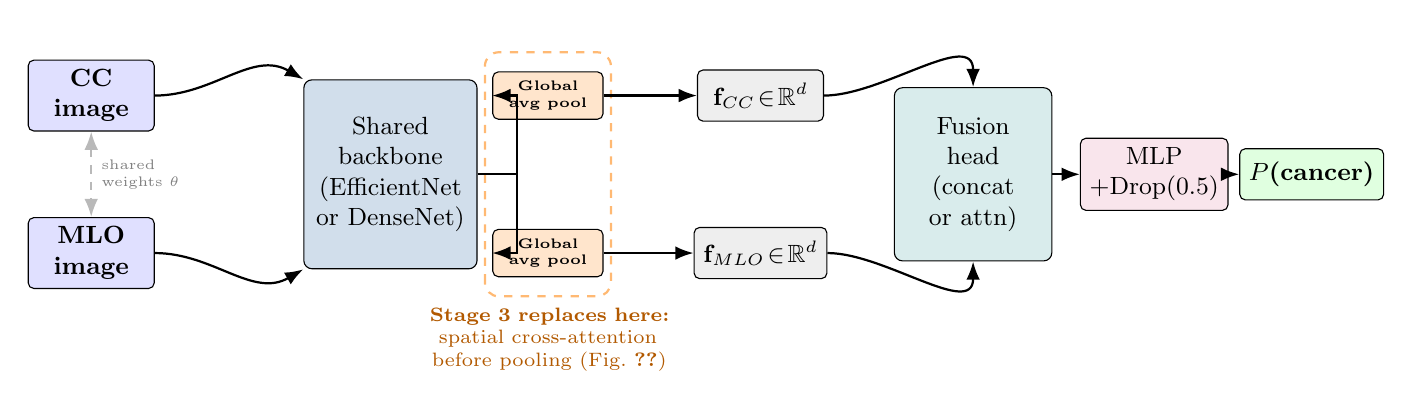
\begin{tikzpicture}[
  imgb/.style={draw, fill=blue!12, rounded corners=2pt,
               minimum width=1.6cm, minimum height=0.8cm, font=\small\bfseries, align=center},
  netb/.style={draw, fill=radblue!18, rounded corners=3pt,
               minimum width=2.2cm, minimum height=2.4cm, font=\small, align=center},
  gapb/.style={draw, fill=orange!20, rounded corners=2pt,
               minimum width=1.4cm, minimum height=0.6cm, font=\tiny\bfseries, align=center},
  featb/.style={draw, fill=gray!13, rounded corners=2pt,
                minimum width=1.6cm, minimum height=0.65cm, font=\small, align=center},
  fusb/.style={draw, fill=teal!15, rounded corners=3pt,
               minimum width=2.0cm, minimum height=2.2cm, font=\small, align=center},
  mlpb/.style={draw, fill=purple!10, rounded corners=2pt,
               minimum width=1.5cm, minimum height=0.65cm, font=\small, align=center},
  outb/.style={draw, fill=green!12, rounded corners=2pt,
               minimum width=1.6cm, minimum height=0.65cm, font=\small\bfseries, align=center},
  arr/.style={->, >=Latex, thick},
]
% Input images
\node[imgb] (cc)  at (0,  1.0) {CC\\image};
\node[imgb] (mlo) at (0, -1.0) {MLO\\image};

% Shared backbone
\node[netb] (bb) at (3.8, 0) {Shared\\backbone\\(EfficientNet\\or DenseNet)};

% Shared-weight annotation between inputs
\draw[<->, dashed, gray!55, >=Latex, thick]
  (cc.south) -- node[right, font=\tiny, gray, align=left] {shared\\weights $\theta$} (mlo.north);

% GAP boxes (explicit, highlighted — this is the key Stage 2 design choice)
\node[gapb] (gap_cc)  at (5.8,  1.0) {Global\\avg pool};
\node[gapb] (gap_mlo) at (5.8, -1.0) {Global\\avg pool};

% Dashed region highlighting GAP as the Stage 2 design choice
\draw[dashed, orange!55, thick, rounded corners=5pt]
  (5.0, -1.55) rectangle (6.6, 1.55);
\node[font=\scriptsize, orange!70!black, align=center, text width=3cm] at (5.8, -2.1)
  {\textbf{Stage~3 replaces here:}\\spatial cross-attention\\before pooling (Fig.~\ref{fig:crossview-arch})};

% Feature vectors
\node[featb] (fcc)  at (8.5,  1.0) {$\mathbf{f}_{CC}\!\in\!\mathbb{R}^d$};
\node[featb] (fmlo) at (8.5, -1.0) {$\mathbf{f}_{MLO}\!\in\!\mathbb{R}^d$};

% Fusion head
\node[fusb] (fus) at (11.2, 0) {Fusion\\head\\(concat\\or attn)};

% MLP
\node[mlpb] (mlp) at (13.5, 0) {MLP\\+Drop(0.5)};

% Output
\node[outb] (out) at (15.5, 0) {$P$(cancer)};

% Arrows: inputs → backbone
\draw[arr] (cc.east)  to[out=0, in=150] (bb.north west);
\draw[arr] (mlo.east) to[out=0, in=210] (bb.south west);

% Arrows: backbone → GAP
\draw[arr] (bb.east) -- +(0.5, 0) |- (gap_cc.west);
\draw[arr] (bb.east) -- +(0.5, 0) |- (gap_mlo.west);

% Arrows: GAP → feature vectors
\draw[arr] (gap_cc.east)  -- (fcc.west);
\draw[arr] (gap_mlo.east) -- (fmlo.west);

% Arrows: features → fusion
\draw[arr] (fcc.east)  to[out=0, in=90]  (fus.north);
\draw[arr] (fmlo.east) to[out=0, in=270] (fus.south);

% Arrows: fusion → MLP → output
\draw[arr] (fus.east) -- (mlp.west);
\draw[arr] (mlp.east) -- (out.west);

\end{tikzpicture}
\caption{BreastPairNet architecture (Stage~2 of \mamnet{}). CC and MLO images from the same breast pass through a \emph{shared} CNN backbone (weights $\theta$ tied for both views). Each view is independently reduced to a global-average-pooled (GAP) feature vector $\mathbf{f}\in\mathbb{R}^d$; the two vectors are fused by concatenation or attention, then classified by a two-layer MLP with 50\% dropout. The orange dashed box highlights the GAP step — the key design decision that Stage~3 (CrossView Transformer, \autoref{fig:crossview-arch}) replaces with bidirectional spatial cross-attention applied \emph{before} pooling.}
\label{fig:breastpairnet-arch}
\end{figure*}

\subsection{CrossView Transformer (Stage 3)}

Replaces global-pooled fusion with spatial cross-attention. Both views pass through the shared CNN backbone to the last spatial feature map; spatial tensors are flattened to tokens and entered into a two-layer Transformer encoder where queries from each view attend to keys/values of the other. Cross-attended outputs are global-averaged and concatenated for the final classifier. \autoref{fig:crossview-arch} contrasts this with BreastPairNet.

\begin{figure*}[tbp]
\centering
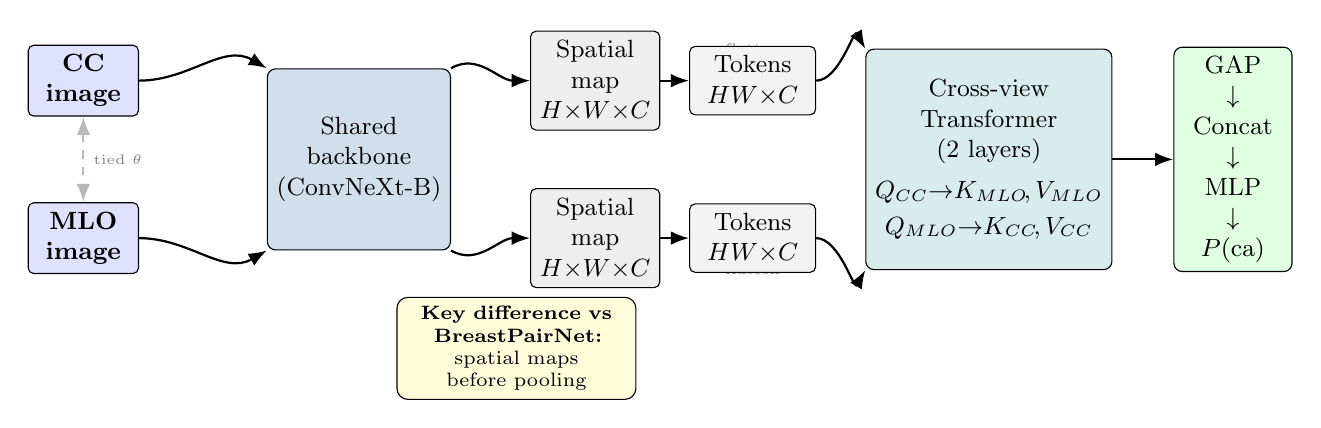
\begin{tikzpicture}[
  imgb/.style={draw, fill=blue!12, rounded corners=2pt,
               minimum width=1.4cm, minimum height=0.75cm, font=\small\bfseries, align=center},
  netb/.style={draw, fill=radblue!18, rounded corners=3pt,
               minimum width=2.0cm, minimum height=2.3cm, font=\small, align=center},
  mapb/.style={draw, fill=gray!13, rounded corners=2pt,
               minimum width=1.5cm, minimum height=0.65cm, font=\small, align=center},
  attnb/.style={draw, fill=teal!15, rounded corners=3pt,
                minimum width=2.2cm, minimum height=2.8cm, font=\small, align=center},
  outb/.style={draw, fill=green!12, rounded corners=3pt,
               minimum width=1.5cm, minimum height=2.0cm, font=\small, align=center},
  arr/.style={->, >=Latex, thick},
]
% Input images
\node[imgb] (cc)  at (0,  1.0) {CC\\image};
\node[imgb] (mlo) at (0, -1.0) {MLO\\image};

% Shared backbone (tall box)
\node[netb] (bb) at (3.5, 0) {Shared\\backbone\\(ConvNeXt-B)};

% Spatial feature maps
\node[mapb] (sm_cc)  at (6.5,  1.0) {Spatial\\map\\$H{\times}W{\times}C$};
\node[mapb] (sm_mlo) at (6.5, -1.0) {Spatial\\map\\$H{\times}W{\times}C$};

% Flatten annotation
\node[font=\tiny, gray] at (8.5,  1.4) {flatten};
\node[font=\tiny, gray] at (8.5, -1.4) {flatten};

% Token sequences
\node[mapb, fill=gray!10, minimum width=1.6cm] (tok_cc)  at (8.5,  1.0) {Tokens\\$HW{\times}C$};
\node[mapb, fill=gray!10, minimum width=1.6cm] (tok_mlo) at (8.5, -1.0) {Tokens\\$HW{\times}C$};

% Cross-attention Transformer
\node[attnb] (attn) at (11.5, 0) {Cross-view\\Transformer\\(2 layers)\\[0.4em]
  $Q_{CC}{\rightarrow}K_{MLO}\!,V_{MLO}$\\[0.2em]
  $Q_{MLO}{\rightarrow}K_{CC}\!,V_{CC}$};

% Output
\node[outb] (out) at (14.6, 0) {GAP\\$\downarrow$\\Concat\\$\downarrow$\\MLP\\$\downarrow$\\$P$(ca)};

% Shared-weight dashed arrow
\draw[<->, dashed, gray!55, >=Latex, thick]
  (cc.south) -- node[right, font=\tiny, gray] {tied $\theta$} (mlo.north);

% Arrows
\draw[arr] (cc.east)  to[out=0, in=150] (bb.north west);
\draw[arr] (mlo.east) to[out=0, in=210] (bb.south west);

\draw[arr] (bb.north east) to[out=30,  in=180] (sm_cc.west);
\draw[arr] (bb.south east) to[out=-30, in=180] (sm_mlo.west);

\draw[arr] (sm_cc)  -- (tok_cc);
\draw[arr] (sm_mlo) -- (tok_mlo);

\draw[arr] (tok_cc.east)  to[out=0, in=120] (attn.north west);
\draw[arr] (tok_mlo.east) to[out=0, in=240] (attn.south west);

\draw[arr] (attn.east) -- (out.west);

% Key difference annotation
\node[font=\scriptsize, draw, rounded corners, fill=yellow!15, align=center,
      text width=2.8cm] at (5.5, -2.4)
  {\textbf{Key difference vs BreastPairNet:}\\spatial maps before pooling};
\end{tikzpicture}
\caption{CrossView Transformer architecture (Stage~3). Unlike BreastPairNet, the backbone output is \emph{not} global-averaged before fusion. Spatial feature maps are flattened to token sequences; a two-layer Transformer encoder applies bidirectional cross-attention ($Q_{CC}$ attends to $K,V$ from MLO and vice versa), enabling the model to localise spatially consistent findings across views before pooling. Best: ConvNeXt-Base, AUROC=0.8317.}
\label{fig:crossview-arch}
\end{figure*}

\subsection{Bounding-box Annotation (Stage 3b)}

Ground-truth boxes (\vindr{}) were drawn as white outlines (40-px line width) on training images only. For \rsna{}, a YOLOv8s detector pre-trained on \vindr{} was used (0.8\% sensitivity --- noisy hints only). Test sets always used original unannotated PNGs to prevent label leakage.

\subsection{MC Dropout (Stage 4)}

MC Dropout was chosen for uncertainty quantification because it requires no architectural modifications: dropout layers that are normally disabled at test time are kept active, converting a single point prediction into a distribution over outputs without retraining \cite{13}. This makes entropy-based case ranking possible at negligible computational cost.

Concretely, BatchNorm is kept in eval mode while dropout remains active. $N=20$ stochastic forward passes per test pair yield probabilities $\{p_i\}_{i=1}^{20}$; their mean $\bar{p}$ is used for classification and the binary entropy $H(\bar{p})=-\bar{p}\log\bar{p}-(1-\bar{p})\log(1-\bar{p})$ quantifies predictive uncertainty. The classification threshold is selected by maximising Youden's~J index ($J = \text{sensitivity} + \text{specificity} - 1$) on the validation set.

\subsection{Hybrid Triage (Stage 6)}

Following Verboom et al.\ \cite{12}, cases are sorted by ascending predictive entropy; the K most-confident fraction is routed to AI and the remainder to a radiologist (modelled as oracle or 85\% sensitivity). Overall sensitivity = (TP$_\text{AI}$ + cancers referred) / total cancers.

\subsection{Training and evaluation}

All models trained on NVIDIA RTX 5070 (12\,GB VRAM) with FP16 mixed-precision (AMP) and AdamW (weight decay 1e-4 for Stage~1; 1e-3 for Stage~2). Primary metric: AUROC. Also reported: F1 at Youden threshold, sensitivity, specificity, \textbf{\satninety{}} (sensitivity at 90\% specificity), and \textbf{PPV} (positive predictive value, precision at the Youden-optimal threshold). 95\% percentile bootstrap confidence intervals ($n$=2000 resamples) on the 2,000-pair test split (99 cancer-positive). Typical AUROC CI width: $\pm$0.04--0.05. Because all models are evaluated on the same 2,000 test pairs, paired bootstrap resampling is more statistically powerful than independent CIs for head-to-head model comparisons.

\section{Experiments and Results}

\subsection{Stage 1 --- Single-view CNN baselines}

DenseNet-121 achieves the best AUROC (0.7564) but only 24.8\% sensitivity at the default threshold (\autoref{tab:single-view}; \autoref{fig:stage1-bar}). All five models overfit (train F1~$\approx$~0.98) and reach only 40--45\% sensitivity at the 90\%-specificity operating point --- well below the $\sim$85\% radiologist sensitivity in screening literature \cite{17}.

\begin{table*}[tbp]
\centering
\caption{Single-view CNN baselines on \vindr{} (n=16,000 train, n=4,000 test images).}
\label{tab:single-view}
\begin{tabular}{@{}p{0.22\textwidth} p{0.10\textwidth} p{0.10\textwidth} p{0.10\textwidth} p{0.08\textwidth} p{0.10\textwidth} p{0.10\textwidth}@{}}
\toprule
Architecture & Image size & Sensitivity & Specificity & F1 & AUROC & S@90\% \\
\midrule
VGG19 & 224 px & 0.2626 & 0.9835 & 0.3323 & 0.7066 & 0.3990 \\
ResNet-50 & 224 px & 0.2677 & 0.9847 & 0.3430 & 0.7286 & 0.4495 \\
EfficientNet-B3 & 224 px & 0.2980 & 0.9687 & 0.3138 & 0.7330 & 0.3990 \\
ResNet-50 (384 px) & 384 px & 0.2879 & 0.9821 & 0.3529 & 0.7489 & 0.4495 \\
\textbf{DenseNet-121} & \textbf{224 px} & \textbf{0.2475} & \textbf{0.9882} & \textbf{0.3356} & \textbf{0.7564} & \textbf{0.4444} \\
\bottomrule
\end{tabular}
\end{table*}

\begin{figure*}[tbp]
\centering
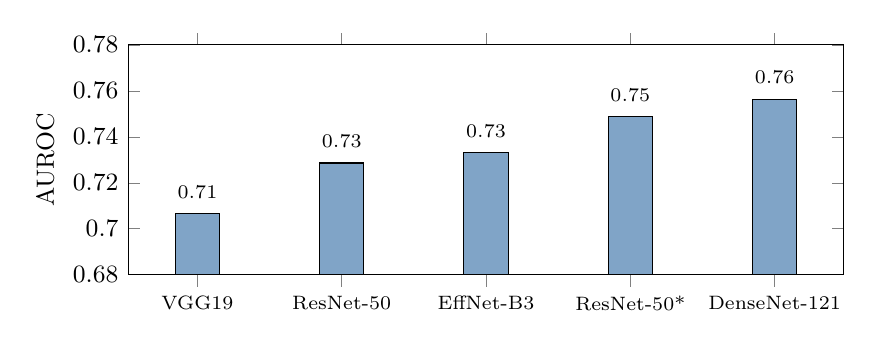
\begin{tikzpicture}
\begin{axis}[
    ybar, bar width=16pt,
    width=0.88\linewidth, height=4.5cm,
    ylabel={AUROC}, ymin=0.68, ymax=0.78,
    ytick={0.68,0.70,0.72,0.74,0.76,0.78},
    xtick=data,
    symbolic x coords={VGG19, ResNet-50, EffNet-B3, ResNet-50*, DenseNet-121},
    xticklabel style={font=\scriptsize},
    nodes near coords, nodes near coords align={vertical},
    every node near coord/.append style={font=\scriptsize, yshift=2pt},
    enlarge x limits=0.12,
]
\addplot[fill=radblue!50] coordinates {
    (VGG19,        0.7066)
    (ResNet-50,    0.7286)
    (EffNet-B3,    0.7330)
    (ResNet-50*,   0.7489)
    (DenseNet-121, 0.7564)
};
\end{axis}
\end{tikzpicture}
\caption{Stage~1: AUROC by single-view architecture. ResNet-50* uses 384\,px; all others 224\,px.}
\label{fig:stage1-bar}
\end{figure*}

\FloatBarrier
\subsection{Stage 2 --- Multi-view BreastPairNet}

The best single model is \textbf{EfficientNet-B3 + attention + +reg} at AUROC=0.8256 (95\% CI 0.7755--0.8707), a +9.1\% relative gain over DenseNet-121 single-view (\autoref{tab:breastpairnet}). Each row in \autoref{tab:breastpairnet} reports the best-checkpoint result from a single training run evaluated on the held-out test split. Standard deviations across runs are not reported as each configuration was trained once; the 95\% percentile bootstrap CIs quantify test-split sampling variability, not run-to-run variability.

\begin{table*}[tbp]
\centering
\caption{BreastPairNet ablation across backbone, fusion, and resolution.}
\label{tab:breastpairnet}
\begin{tabular}{@{}p{0.20\textwidth} p{0.08\textwidth} p{0.07\textwidth} p{0.18\textwidth} p{0.06\textwidth} p{0.06\textwidth} p{0.05\textwidth} p{0.15\textwidth}@{}}
\toprule
Architecture & Fusion & Image & Best AUROC [95\% CI] & F1 & Sens & PPV & S@90\% [95\% CI] \\
\midrule
ResNet-50 & concat & 384 px & 0.7467 [0.6921--0.7998] & 0.2350 & 0.5354 & 0.151 & 0.4646 [0.3736--0.5673] \\
ResNet-50 & attention & 224 px & 0.7847 [0.7324--0.8338] & 0.2522 & 0.5859 & 0.161 & 0.5051 [0.4023--0.6019] \\
ResNet-50 & attention & 512 px & 0.7922 [0.7339--0.8429] & 0.2093 & 0.7475 & 0.122 & 0.5152 [0.4130--0.6214] \\
ResNet-50 & concat & 224 px & 0.7962 [0.7428--0.8445] & 0.2363 & 0.6970 & 0.142 & 0.4949 [0.3958--0.5977] \\
DenseNet-121 & attention & 224 px & 0.8014 [0.7487--0.8515] & 0.2800 & 0.6364 & 0.179 & 0.5758 [0.4660--0.6667] \\
EfficientNet-B3 & attention & 224 px & 0.8048 [0.7530--0.8556] & 0.2138 & 0.7677 & 0.124 & 0.5455 [0.4476--0.6449] \\
DenseNet-121 & concat & 224 px & 0.8073 [0.7577--0.8504] & 0.2101 & 0.7374 & 0.122 & 0.5152 [0.4141--0.6100] \\
DenseNet-121 \textbf{+reg} & attention & 224 px & 0.8097 [0.7594--0.8591] & 0.2033 & 0.7980 & 0.117 & 0.5556 [0.4301--0.6458] \\
DenseNet-121 & attention & 512 px & 0.8150 [0.7675--0.8617] & 0.1928 & 0.8081 & 0.109 & 0.5455 [0.4476--0.6408] \\
DenseNet-121 \textbf{+reg} & concat & 224 px & 0.8177 [0.7659--0.8649] & 0.2357 & 0.7677 & 0.139 & 0.6061 [0.5047--0.7000] \\
EfficientNet-B3 & attention & 512 px & 0.8175 [0.7698--0.8661] & 0.2807 & 0.7273 & 0.160 & 0.5556 [0.4495--0.6505] \\
\textbf{EfficientNet-B3 +reg} & \textbf{attention} & \textbf{224 px} & \textbf{0.8256 [0.7755--0.8707]} & \textbf{0.3701} & \textbf{0.6263} & \textbf{0.263} & \textbf{0.6263 [0.5229--0.7143]} \\
\bottomrule
\multicolumn{8}{@{}p{0.96\textwidth}@{}}{\small PPV = TP/(TP+FP) at the Youden-optimal threshold. At 4.95\% prevalence, PPV is inherently low; higher PPV reflects a more conservative threshold (lower sensitivity). All CIs via 2,000-resample percentile bootstrap on the 2,000-pair test split.}
\end{tabular}
\end{table*}

\begin{table*}[tbp]
\centering
\caption{Isolated effect of the +reg training recipe.}
\label{tab:regularisation-effect}
\begin{tabular}{@{}llccc@{}}
\toprule
Backbone & Fusion & Base AUROC & +reg AUROC & Gain \\
\midrule
DenseNet-121 & concat & 0.8073 & 0.8177 & +0.010 \\
DenseNet-121 & attention & 0.8014 & 0.8097 & +0.008 \\
EfficientNet-B3 & attention & 0.8048 & \textbf{0.8256} & \textbf{+0.021} \\
\bottomrule
\end{tabular}
\end{table*}

\begin{figure*}[tbp]
\centering
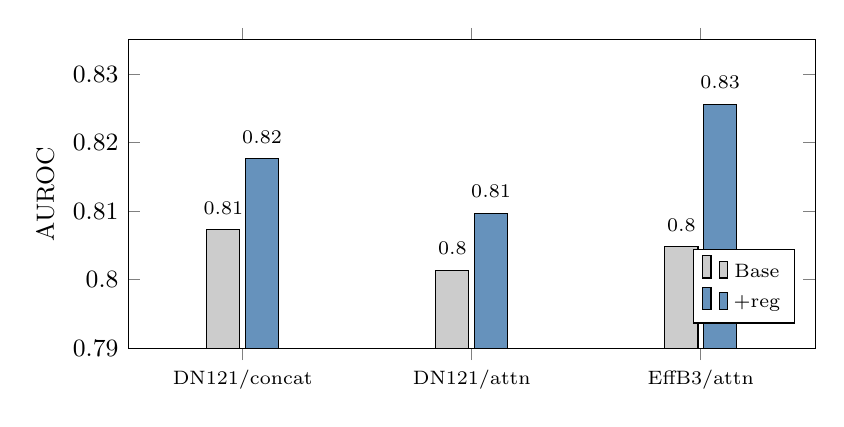
\begin{tikzpicture}
\begin{axis}[
    ybar, bar width=12pt,
    width=0.85\linewidth, height=5.5cm,
    ylabel={AUROC}, ymin=0.79, ymax=0.835,
    ytick={0.79,0.80,0.81,0.82,0.83},
    xtick=data,
    symbolic x coords={DN121/concat, DN121/attn, EffB3/attn},
    xticklabel style={font=\scriptsize},
    legend style={at={(0.97,0.08)}, anchor=south east, font=\scriptsize},
    nodes near coords, nodes near coords align={vertical},
    every node near coord/.append style={font=\scriptsize, yshift=2pt},
    enlarge x limits=0.25,
]
\addplot[fill=gray!40] coordinates {
    (DN121/concat, 0.8073)(DN121/attn, 0.8014)(EffB3/attn, 0.8048)
};
\addplot[fill=radblue!60] coordinates {
    (DN121/concat, 0.8177)(DN121/attn, 0.8097)(EffB3/attn, 0.8256)
};
\legend{Base, {+reg}}
\end{axis}
\end{tikzpicture}
\caption{Stage~2: Effect of +reg on AUROC for three backbone/fusion pairs.}
\label{fig:stage2-reg-bar}
\end{figure*}

All point estimates in \autoref{tab:breastpairnet} and \autoref{tab:crossview} are obtained by re-evaluating each best-checkpoint model on the held-out test split (n=2,000 pairs, 99 positives) at the Youden-optimal threshold, with 95\% percentile bootstrap confidence intervals ($n$=2,000 resamples). Validation AUROC curves for the best Stage~2 and Stage~3 models are shown in \autoref{fig:training-curves}.

Three observations stand out (\autoref{tab:regularisation-effect}; \autoref{fig:stage2-reg-bar}). \textbf{(i) +reg consistently lifts AUROC} by from 0.008 to 0.021 across all backbone/fusion pairs. \textbf{(ii) Resolution scaling is not uniformly beneficial}: DenseNet-121 benefits from 512\,px (+0.014), but EfficientNet-B3 +reg at 224\,px (0.8256) beats 512\,px without +reg (0.8175). \textbf{(iii) ResNet-50 degrades at 384\,px} (0.7467 vs 0.7962 at 224\,px) due to batch-size reduction under VRAM pressure.

\begin{figure*}[tbp]
\centering
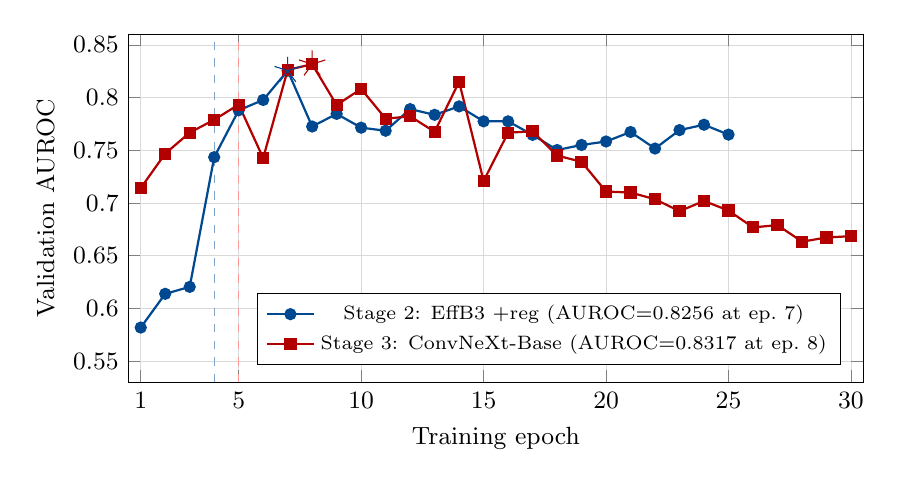
\begin{tikzpicture}
\begin{axis}[
    width=0.9\linewidth, height=6cm,
    xlabel={Training epoch}, ylabel={Validation AUROC},
    xmin=0.5, xmax=30.5, ymin=0.53, ymax=0.86,
    xtick={1,5,10,15,20,25,30},
    ytick={0.55,0.60,0.65,0.70,0.75,0.80,0.85},
    legend style={at={(0.97,0.05)}, anchor=south east, font=\scriptsize},
    grid=both, grid style={line width=0.2pt, draw=gray!30},
    mark size=1.8pt,
]
% BreastPairNet EffB3 +reg (Stage 2 best)
\addplot[radblue, mark=*, thick] coordinates {
    (1,0.5819)(2,0.6139)(3,0.6205)
    (4,0.7435)(5,0.7880)(6,0.7978)(7,0.8256)
    (8,0.7726)(9,0.7846)(10,0.7715)(11,0.7686)(12,0.7891)
    (13,0.7837)(14,0.7917)(15,0.7775)(16,0.7775)(17,0.7647)
    (18,0.7503)(19,0.7551)(20,0.7584)(21,0.7674)(22,0.7517)
    (23,0.7692)(24,0.7743)(25,0.7649)
};
% CrossView ConvNeXt-Base (Stage 3 best)
\addplot[red!70!black, mark=square*, thick] coordinates {
    (1,0.7142)(2,0.7469)(3,0.7668)(4,0.7790)
    (5,0.7934)(6,0.7427)(7,0.8263)(8,0.8317)
    (9,0.7930)(10,0.8083)(11,0.7800)(12,0.7823)(13,0.7676)
    (14,0.8151)(15,0.7210)(16,0.7667)(17,0.7681)(18,0.7451)
    (19,0.7391)(20,0.7109)(21,0.7100)(22,0.7036)(23,0.6923)
    (24,0.7020)(25,0.6929)(26,0.6769)(27,0.6791)(28,0.6634)
    (29,0.6673)(30,0.6686)
};
% Stars at best epochs
\addplot[only marks, mark=star, mark size=5pt, radblue, forget plot]
    coordinates {(7,0.8256)};
\addplot[only marks, mark=star, mark size=5pt, red!70!black, forget plot]
    coordinates {(8,0.8317)};
% Vertical dashed line: EffB3 backbone unfreeze (epoch 4)
\addplot[dashed, radblue!50, thin, forget plot] coordinates {(4,0.53)(4,0.86)};
% Vertical dashed line: ConvNeXt backbone unfreeze (epoch 5)
\addplot[dashed, red!40, thin, forget plot] coordinates {(5,0.53)(5,0.86)};
\legend{Stage 2: EffB3 +reg (AUROC=0.8256 at ep.~7), Stage 3: ConvNeXt-Base (AUROC=0.8317 at ep.~8)}
\end{axis}
\end{tikzpicture}
\caption{Validation AUROC vs.\ training epoch for the best Stage~2 (EffB3 +reg) and Stage~3 (ConvNeXt-Base) models. Vertical dashed lines mark the backbone unfreeze point (epoch~4 for EffB3, epoch~5 for ConvNeXt). Stars ($\star$) indicate the best-checkpoint epoch used for test-set evaluation. Both models overfit after their best epoch as training loss continues to decrease while validation AUROC plateaus.}
\label{fig:training-curves}
\end{figure*}

\FloatBarrier
\subsection{Stage 3 --- CrossView Transformer}

\subsubsection{Performance without annotation}

\begin{table*}[tbp]
\centering
\caption{CrossView Transformer results without bounding-box annotation.}
\label{tab:crossview}
{\small\setlength{\tabcolsep}{4pt}%
\begin{tabular}{@{}p{0.19\textwidth} p{0.10\textwidth} p{0.20\textwidth} p{0.06\textwidth} p{0.06\textwidth} p{0.06\textwidth} p{0.20\textwidth}@{}}
\toprule
Architecture & Training data & Best AUROC [95\% CI] & F1 & Sens & PPV & S@90\% [95\% CI] \\
\midrule
DenseNet-121 (medical init) & VinDr & 0.7648 [0.7116--0.8210] & 0.2374 & 0.5960 & 0.148 & 0.5051 [0.4020--0.6100] \\
EfficientNet-B3 & VinDr & 0.7795 [0.7276--0.8300] & 0.2022 & 0.7273 & 0.117 & 0.4545 [0.3474--0.5500] \\
DenseNet-121 & VinDr & 0.7874 [0.7299--0.8401] & 0.2678 & 0.6465 & 0.169 & 0.5556 [0.4474--0.6482] \\
DenseNet-121 & VinDr+RSNA & 0.8028 [0.7484--0.8536] & 0.2640 & 0.6667 & 0.165 & 0.5354 [0.4433--0.6404] \\
\textbf{ConvNeXt-Base} & \textbf{VinDr} & \textbf{0.8317 [0.7832--0.8753]} & \textbf{0.2587} & \textbf{0.7475} & \textbf{0.156} & \textbf{0.5758 [0.4737--0.6768]} \\
\bottomrule
\end{tabular}}
\end{table*}

\textbf{ConvNeXt-Base} achieves the best AUROC at 0.8317 (+10.0\% over single-view DenseNet-121). DenseNet-121 with \vindr{}+\rsna{} joint training reaches AUROC=0.8028, confirming incremental cross-dataset benefit. Chest-X-ray pretraining via the torchxrayvision library\footnote{torchxrayvision: \texttt{github.com/mlmed/torchxrayvision}} underperforms ImageNet initialisation (AUROC 0.7648 vs 0.7874), consistent with domain mismatch between lung radiographs and mammographic texture.

\subsubsection{Bounding-box annotation ablation}

\begin{table*}[tbp]
\centering
\caption{Bounding-box annotation ablation. Test set always uses original unannotated PNGs.}
\label{tab:annotation-ablation}
\begin{tabular}{@{}p{0.23\textwidth} p{0.27\textwidth} p{0.27\textwidth} p{0.10\textwidth}@{}}
\toprule
Architecture & No annotation AUROC [95\% CI] & With annotation AUROC [95\% CI] & \(\Delta\)AUROC \\
\midrule
DenseNet-121 & 0.7874 [0.7299--0.8401] & 0.5862 [0.5274--0.6433] & -0.201 \\
DenseNet-121 +RSNA & 0.8028 [0.7484--0.8536] & 0.6675 & -0.135 \\
DenseNet-121 (medical) & 0.7648 [0.7116--0.8210] & 0.6433 [0.5886--0.6966] & -0.122 \\
EfficientNet-B3 & 0.7795 [0.7276--0.8300] & 0.6020 [0.5460--0.6617] & -0.178 \\
\bottomrule
\end{tabular}
\end{table*}

\begin{figure*}[tbp]
\centering
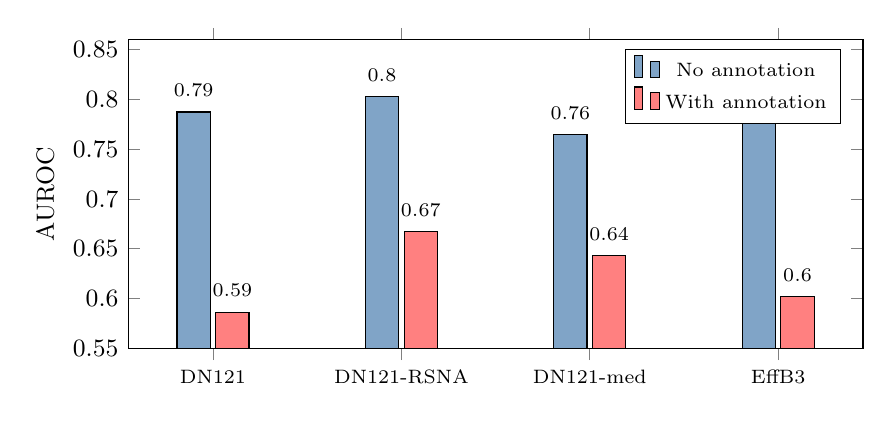
\begin{tikzpicture}
\begin{axis}[
    ybar, bar width=12pt,
    width=0.9\linewidth, height=5.5cm,
    ylabel={AUROC}, ymin=0.55, ymax=0.86,
    ytick={0.55,0.60,0.65,0.70,0.75,0.80,0.85},
    xtick=data,
    symbolic x coords={DN121, DN121-RSNA, DN121-med, EffB3},
    xticklabel style={font=\scriptsize},
    legend style={at={(0.97,0.97)}, anchor=north east, font=\scriptsize},
    nodes near coords, nodes near coords align={vertical},
    every node near coord/.append style={font=\scriptsize, yshift=2pt},
    enlarge x limits=0.15,
]
\addplot[fill=radblue!50] coordinates {
    (DN121, 0.7874)(DN121-RSNA, 0.8028)(DN121-med, 0.7648)(EffB3, 0.7795)
};
\addplot[fill=red!50] coordinates {
    (DN121, 0.5862)(DN121-RSNA, 0.6675)(DN121-med, 0.6433)(EffB3, 0.6020)
};
\legend{No annotation, With annotation}
\end{axis}
\end{tikzpicture}
\caption{Stage~3b: Annotation consistently degrades AUROC due to shortcut learning and test-time distribution shift.}
\label{fig:annotation-bar}
\end{figure*}

\textbf{All four pairs show annotation consistently degrades AUROC by 0.122--0.201} (\autoref{tab:annotation-ablation}; \autoref{fig:annotation-bar}). At epoch 4 the backbone unfreezes and fits the white box outlines as a shortcut texture; training F1 reaches $\sim$0.97 while test AUROC collapses because boxes are absent at test time. Potential remedies may include: (a) box-dropout regularisation, in which annotation boxes are randomly masked during training to prevent over-reliance on the shortcut; (b) test-time box injection via a lesion detector, so the test distribution matches training; or (c) cropping the input to the bounding-box region, passing only the annotated content to the model rather than the full image with a drawn outline. These suggestions are speculative; we are not aware of published evidence validating them specifically for mammography annotation shortcuts.

\FloatBarrier
\subsection{Stage 4 --- MC Dropout uncertainty quantification}

\begin{table}[htbp]
\centering
\caption{MC Dropout vs deterministic inference (DenseNet-121/concat).}
\label{tab:mc-dropout}
{\footnotesize\setlength{\tabcolsep}{3pt}%
\begin{tabular}{@{}p{1.9cm}ccccc@{}}
\toprule
Mode & AUROC & Sens & Spec & S@90\% & Thr. \\
\midrule
Deterministic & 0.8073 & 0.7374 & 0.7249 & 0.5152 & 0.3304 \\
\textbf{MC Dropout} & \textbf{0.8099} & \textbf{0.7677} & \textbf{0.7007} & \textbf{0.5253} & \textbf{0.3138} \\
\bottomrule
\end{tabular}}
\end{table}

MC Dropout slightly improves AUROC (+0.003) and produces a meaningful sensitivity shift (+3.0 percentage points, \autoref{tab:mc-dropout}; inference flow in \autoref{fig:mc-dropout-flow}). More importantly, the mean entropy is \textbf{0.5670} on cancer-positive pairs versus \textbf{0.5112} on negatives (\autoref{tab:mc-entropy}) --- a 0.056-nat gap that enables the Stage~6 triage policy.

\begin{table}[htbp]
\centering
\caption{Predictive entropy by class ($N=20$ MC passes, 2,000 test pairs).}
\label{tab:mc-entropy}
\begin{tabular}{@{}lcc@{}}
\toprule
Entropy & Negatives ($n=1{,}901$) & Positives ($n=99$) \\
\midrule
Mean    & 0.5112 & 0.5670 \\
Median  & 0.5310 & 0.6221 \\
Std dev & 0.1436 & 0.1370 \\
\midrule
\multicolumn{3}{@{}p{0.9\columnwidth}@{}}{\small Gap: $+$0.056 nats. Higher entropy $\Rightarrow$ refer high-uncertainty cases.} \\
\bottomrule
\end{tabular}
\end{table}

\begin{figure*}[tbp]
\centering
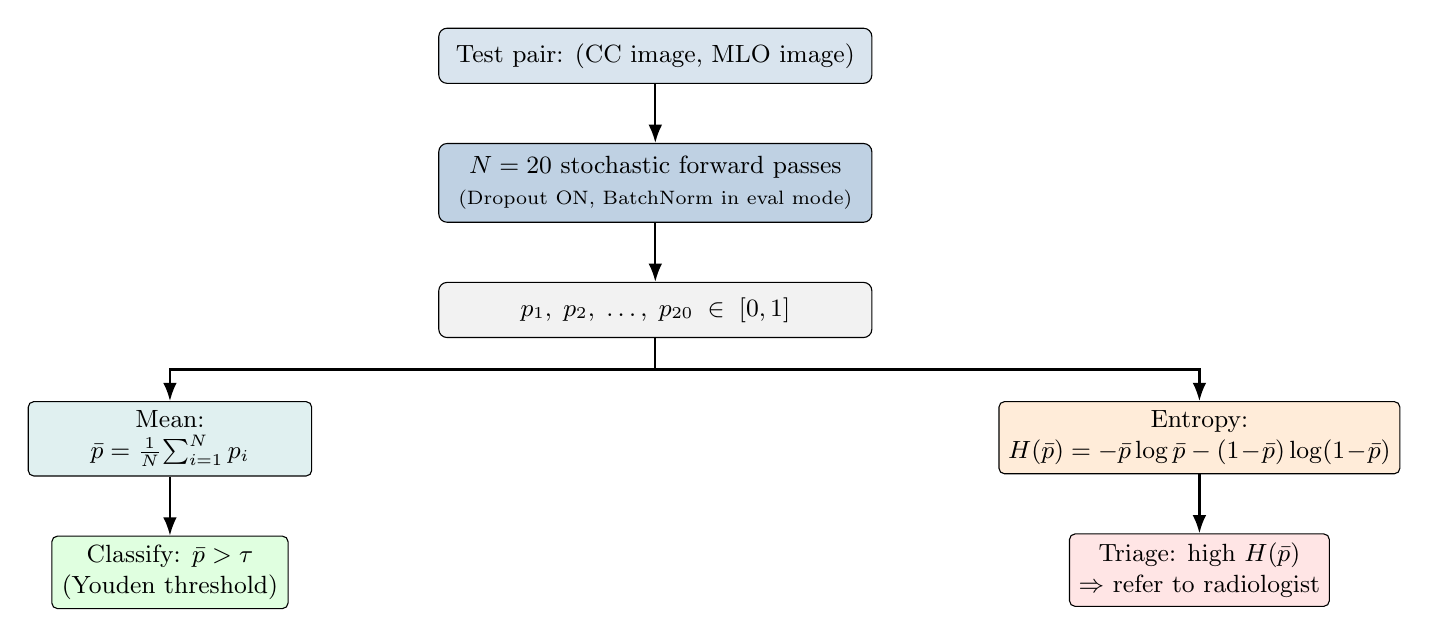
\begin{tikzpicture}[
  mainb/.style={draw, fill=radblue!15, rounded corners=3pt,
                minimum width=5.5cm, minimum height=0.7cm, font=\small, align=center},
  passb/.style={draw, fill=gray!10, rounded corners=2pt,
                minimum width=3.2cm, minimum height=0.65cm, font=\small, align=center},
  calcb/.style={draw, fill=teal!12, rounded corners=2pt,
                minimum width=3.6cm, minimum height=0.7cm, font=\small, align=center},
  decb/.style={draw, rounded corners=2pt,
               minimum width=3.0cm, minimum height=0.7cm, font=\small, align=center},
  arr/.style={->, >=Latex, thick},
  node distance=0.75cm,
]
% Top: input
\node[mainb] (inp) {Test pair: (CC image, MLO image)};

% Multiple passes -- shown as a box
\node[mainb, fill=radblue!25, minimum height=1.0cm, below=of inp] (passes)
  {$N=20$ stochastic forward passes\\{\scriptsize(Dropout ON, BatchNorm in eval mode)}};

% Probability samples
\node[mainb, fill=gray!10, below=of passes] (probs)
  {$p_1,\; p_2,\; \ldots,\; p_{20} \;\in\; [0,1]$};

% Two outputs side-by-side
\node[calcb, below left=0.8cm and 1.6cm of probs] (meanbox)
  {Mean:\\$\bar{p}=\tfrac{1}{N}\!\sum_{i=1}^{N} p_i$};
\node[calcb, fill=orange!15, below right=0.8cm and 1.6cm of probs] (entbox)
  {Entropy:\\$H(\bar{p})=-\bar{p}\log\bar{p}-(1\!-\!\bar{p})\log(1\!-\!\bar{p})$};

% Decision boxes
\node[decb, fill=green!12, below=of meanbox] (classify)
  {Classify: $\bar{p} > \tau$\\(Youden threshold)};
\node[decb, fill=red!10, below=of entbox] (refer)
  {Triage: high $H(\bar{p})$\\$\Rightarrow$ refer to radiologist};

% Arrows
\draw[arr] (inp)    -- (passes);
\draw[arr] (passes) -- (probs);
\draw[arr] (probs.south) -- +(0,-0.4) -| (meanbox.north);
\draw[arr] (probs.south) -- +(0,-0.4) -| (entbox.north);
\draw[arr] (meanbox) -- (classify);
\draw[arr] (entbox)  -- (refer);
\end{tikzpicture}
\caption{MC Dropout inference (Stage~4). Dropout layers remain active at test time while BatchNorm uses running statistics. Twenty stochastic passes produce a probability distribution $\{p_i\}_{i=1}^{20}$. The mean $\bar{p}$ is used for classification at the Youden-optimal threshold $\tau$; the binary entropy $H(\bar{p})$ ranks cases by epistemic uncertainty and routes high-uncertainty cases to a radiologist in the Stage~6 triage protocol.}
\label{fig:mc-dropout-flow}
\end{figure*}

\FloatBarrier
\subsection{Stage 5 --- Model ensemble}

\subsubsection{Original ensemble (16 BreastPairNet models)}

Mean-probability ensemble of 16 BreastPairNet checkpoints combined with three breast-asymmetry models and five-fold test-time augmentation (TTA$\times$5). \textbf{Best result in the study}: AUROC=0.8458, sensitivity=0.7374, specificity=0.8296, F1=0.2944, S@90\%=0.6566, S@95\%=0.5657 at threshold 0.3414 (TP=73, TN=1577, FP=324, FN=26; \autoref{tab:ensemble}).

\begin{table*}[tbp]
\centering
\caption{Best ensemble result (mean probability, TTA$\times$5).}
\label{tab:ensemble}
\begin{tabular}{@{}p{0.20\textwidth} cccccccc@{}}
\toprule
Method & AUROC & Sens & Spec & F1 & PPV & S@90\% & S@95\% & Threshold \\
\midrule
\textbf{Ensemble (N=16, TTA=5)} & \textbf{0.8458} & \textbf{0.7374} & \textbf{0.8296} & \textbf{0.2944} & \textbf{0.184} & \textbf{0.6566} & \textbf{0.5657} & \textbf{0.3414} \\
\bottomrule
\multicolumn{9}{@{}p{0.96\textwidth}@{}}{\small PPV=0.184 means 1 in 5.4 recalls is cancer-positive at this threshold; at 4.95\% test prevalence, this is consistent with reported breast-cancer AI triage literature (PPV 15--25\%).}
\end{tabular}
\end{table*}

\begin{table}[htbp]
\centering
\caption{Confusion matrix at Youden threshold ($t=0.3414$).}
\label{tab:confusion-matrix}
\begin{tabular}{@{}lcc@{}}
\toprule
 & Pred.\ negative & Pred.\ positive \\
\midrule
Actual negative & TN = 1{,}577 & FP = 324 \\
Actual positive & FN = 26      & TP = 73  \\
\bottomrule
\end{tabular}
\end{table}

The per-class breakdown is shown in \autoref{tab:confusion-matrix}. This ensemble does \textbf{not} include ConvNeXt-Base or EfficientNet-B3 +reg models.

\subsubsection{Updated ensemble (25 checkpoints)}

Adding all CrossView checkpoints (including lower-epoch snapshots) gives AUROC=0.8441, S@90\%=0.6566 (unchanged), sensitivity=0.7677. The marginal AUROC drop confirms that weaker models drag the mean under mean combination; S@90\% is robust.

\subsubsection{Selective ensemble (top-3 +reg + top-5 CrossView + 3 asymmetry)}

11 models, TTA$\times$5: AUROC=0.8446, S@90\%=0.6667 (+0.010 over baseline). Marginally better at the clinical operating point; difference is within sampling noise.

\subsubsection{Ensemble comparison}

\autoref{tab:ensemble-comparison} summarises all three configurations. Full metrics (specificity, F1, threshold) were only computed for the primary 16-model configuration; secondary configurations were evaluated on AUROC and the clinical operating point (S@90\%) only.

\begin{table}[htbp]
\centering
\caption{Comparison of ensemble configurations (TTA$\times$5, mean-probability combination).}
\label{tab:ensemble-comparison}
{\footnotesize\setlength{\tabcolsep}{3pt}%
\begin{tabular}{@{}p{3.2cm}cccc@{}}
\toprule
Configuration & Models & AUROC & Sens & S@90\% \\
\midrule
Original (BreastPairNet) & 16 & \textbf{0.8458} & 0.7374 & 0.6566 \\
Updated (+CrossView) & 25 & 0.8441 & 0.7677 & 0.6566 \\
Selective (+reg+CVT+asym) & 11 & 0.8446 & --- & \textbf{0.6667} \\
\bottomrule
\multicolumn{5}{@{}p{0.9\columnwidth}@{}}{\small ---: not evaluated. Differences in AUROC are within the $\pm$0.04 percentile bootstrap CI; the selective ensemble offers marginal S@90\% benefit.}
\end{tabular}}
\end{table}

\FloatBarrier
\subsection{Stage 6 --- Hybrid triage simulation}

\begin{table}[htbp]
\centering
\caption{Hybrid triage sweep (oracle vs.\ 85\% radiologist sensitivity).}
\label{tab:triage-sweep}
{\scriptsize\setlength{\tabcolsep}{2pt}%
\begin{tabular}{@{}lccccc@{}}
\toprule
Frac & Wkld $\Delta$ & Sen (or.) & Sen (85\%r) & AI Sen & Recall \\
\midrule
30\% & -30\% & 0.9495 & 0.8253 & 0.7059 & 0.0017 \\
40\% & -40\% & 0.9192 & 0.8071 & 0.6800 & 0.0013 \\
\textbf{50\%} & \textbf{-50\%} & \textbf{0.8788} & \textbf{0.7727} & \textbf{0.5862} & \textbf{0.0031} \\
60\% & -60\% & 0.8283 & 0.7359 & 0.5526 & 0.0052 \\
70\% & -70\% & 0.7677 & 0.6935 & 0.5400 & 0.0133 \\
80\% & -80\% & 0.7677 & 0.7207 & 0.6618 & 0.1305 \\
90\% & -90\% & 0.7677 & 0.7450 & 0.7262 & 0.2238 \\
\bottomrule
\end{tabular}}
\end{table}

\begin{figure*}[tbp]
\centering
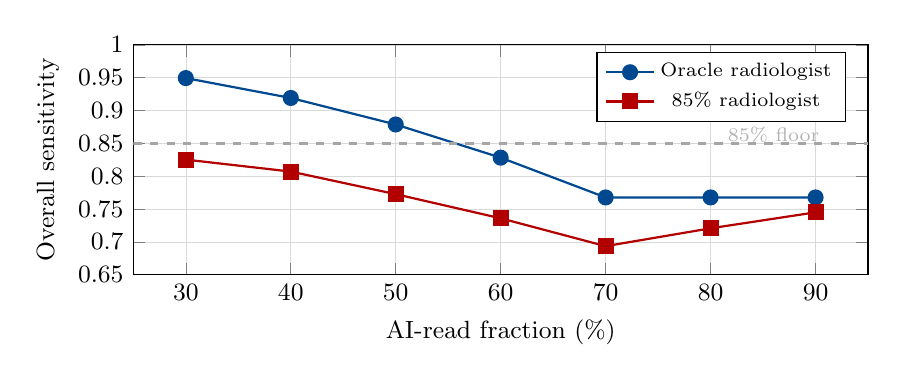
\begin{tikzpicture}
\begin{axis}[
    width=0.9\linewidth, height=4.5cm,
    xlabel={AI-read fraction (\%)},
    ylabel={Overall sensitivity},
    xmin=25, xmax=95, ymin=0.65, ymax=1.00,
    xtick={30,40,50,60,70,80,90},
    ytick={0.65,0.70,0.75,0.80,0.85,0.90,0.95,1.00},
    legend style={at={(0.97,0.97)}, anchor=north east, font=\scriptsize},
    grid=both, grid style={line width=0.2pt, draw=gray!30},
    mark size=2.5pt,
]
\addplot[radblue, mark=*, thick] coordinates {
    (30,0.9495)(40,0.9192)(50,0.8788)(60,0.8283)(70,0.7677)(80,0.7677)(90,0.7677)
};
\addplot[red!70!black, mark=square*, thick] coordinates {
    (30,0.8253)(40,0.8071)(50,0.7727)(60,0.7359)(70,0.6935)(80,0.7207)(90,0.7450)
};
\addplot[dashed, gray!70, thick, forget plot] coordinates {(25,0.85)(95,0.85)};
\node[font=\scriptsize, gray!60] at (axis cs:86,0.863) {85\% floor};
\legend{Oracle radiologist, 85\% radiologist}
\end{axis}
\end{tikzpicture}
\caption{Stage~6: Overall sensitivity vs.\ AI-read fraction. Dashed line = 85\% clinical sensitivity floor.}
\label{fig:triage-sensitivity}
\end{figure*}

Under oracle assumptions, \textbf{K=50\% delivers 87.9\% overall sensitivity with 50\% workload reduction} (\autoref{tab:triage-sweep}; \autoref{fig:triage-sensitivity}). Under realistic 85\% radiologist sensitivity \cite{17}, the same K=50\% yields 77.3\% --- below the clinical floor. Achieving $\geq$80\% overall sensitivity under realistic conditions requires K$\leq$40\% (\autoref{tab:sensitivity-floors}).

\begin{table}[htbp]
\centering
\caption{Max AI-read fraction by sensitivity floor.}
\label{tab:sensitivity-floors}
{\footnotesize\setlength{\tabcolsep}{3pt}%
\begin{tabular}{@{}p{1.7cm}ccp{2.2cm}@{}}
\toprule
Floor & Oracle & 85\% rad & Workload $\Delta$ \\
\midrule
$\geq$90\% & 40\% & n/a & -40\% \\
$\geq$85\% & 50--60\% & n/a & -50\% to -60\% \\
$\geq$80\% & 60\% & 40\% & -40\% to -60\% \\
$\geq$77\% & 70\% & 50\% & -50\% to -70\% \\
\bottomrule
\end{tabular}}
\end{table}

\FloatBarrier
\subsection{Comparison to literature}

\begin{table}[htbp]
\centering
\caption{AUROC progression on \vindr{} binary cancer detection.}
\label{tab:auc-progression}
\begin{tabular}{@{}p{0.62\columnwidth} p{0.28\columnwidth}@{}}
\toprule
Method & AUROC \\
\midrule
MamT4 \cite{18}\(\ddagger\) & 0.840 \\
Ours Stage 1 (DenseNet-121) & 0.7564 \\
Ours Stage 2 (BreastPairNet) & 0.8256 \\
Ours Stage 3 (CrossView) & 0.8317 \\
\textbf{Ours Stage 5 (Ensemble)} & \textbf{0.8458} \\
\bottomrule
\end{tabular}
\end{table}

AUROC progression across the pipeline is summarised in \autoref{tab:auc-progression} and visualised in \autoref{fig:auc-progression}. The $\ddagger$ symbol in \autoref{tab:auc-progression} flags a methodological difference: MamT4 \cite{18} excludes BI-RADS~3 cases from evaluation, while our pipeline retains them as negative, making the AUROC values not directly comparable. McKinney et al. \cite{11} (AUC=0.889) and Yoon et al. \cite{4} (pooled AUC=0.87) report on different datasets and are likewise not directly comparable.

\begin{figure}[tbp]
\centering
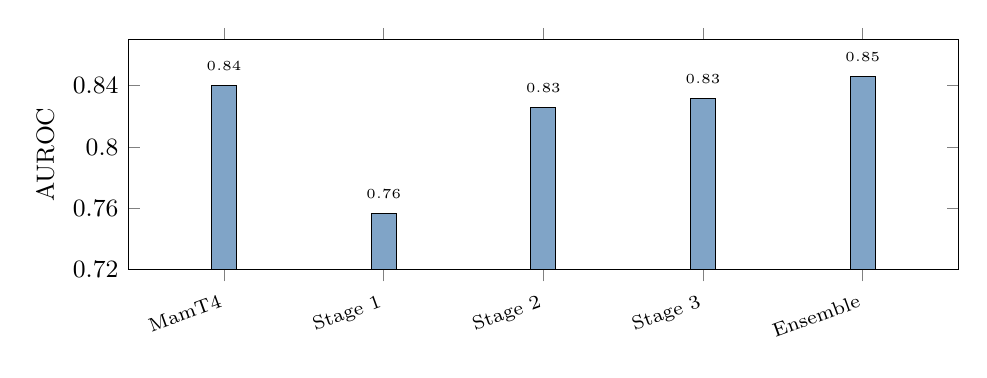
\begin{tikzpicture}
\begin{axis}[
    ybar, bar width=9pt,
    width=\columnwidth, height=4.5cm,
    ylabel={AUROC}, ymin=0.72, ymax=0.87,
    ytick={0.72,0.76,0.80,0.84},
    xtick=data,
    symbolic x coords={MamT4, Stage 1, Stage 2, Stage 3, Ensemble},
    xticklabel style={font=\scriptsize, rotate=20, anchor=north east},
    nodes near coords, nodes near coords align={vertical},
    every node near coord/.append style={font=\tiny, yshift=2pt},
    enlarge x limits=0.15,
]
\addplot[fill=radblue!50] coordinates {
    (MamT4,    0.840)
    (Stage 1,  0.7564)
    (Stage 2,  0.8256)
    (Stage 3,  0.8317)
    (Ensemble, 0.8458)
};
\end{axis}
\end{tikzpicture}
\caption{AUROC progression across pipeline stages vs.\ MamT4 prior work.}
\label{fig:auc-progression}
\end{figure}

\FloatBarrier
\subsection{External validation on \rsna{}}

The best ensemble (AUROC=0.8458 on \vindr{}) was applied zero-shot to \rsna{}. Full metrics are shown in \autoref{tab:external-validation}; the per-metric performance drop is detailed in \autoref{tab:domain-gap}.

\begin{table}[htbp]
\centering
\caption{External validation: \vindr{} (2{,}000 pairs, 99 cancers) vs.\ \rsna{} (4{,}764 pairs, 110 cancers).}
\label{tab:external-validation}
{\scriptsize\setlength{\tabcolsep}{3pt}%
\begin{tabular}{@{}lcccc@{}}
\toprule
Dataset & AUROC [95\% CI] & S@90\% & Sens & Spec \\
\midrule
\vindr{} & 0.8458 & 0.6566 & 0.7374 & 0.8296 \\
\rsna{} & 0.6008 [0.5577--0.6585] & 0.1636 & 0.3909 & 0.7598 \\
\bottomrule
\end{tabular}}
\end{table}

\begin{table}[htbp]
\centering
\caption{Performance drop: \vindr{} $\to$ \rsna{}.}
\label{tab:domain-gap}
{\footnotesize\setlength{\tabcolsep}{3pt}%
\begin{tabular}{@{}p{1.6cm}cccc@{}}
\toprule
Metric & \vindr{} & \rsna{} & Drop & Rel. \\
\midrule
AUROC & 0.8458 & 0.6008 & -0.245 & -29\% \\
S@90\%spec & 0.6566 & 0.1636 & \textbf{-0.493} & \textbf{-75\%} \\
Sensitivity & 0.7374 & 0.3909 & -0.347 & -47\% \\
Specificity & 0.8296 & 0.7598 & -0.070 & -8\% \\
\bottomrule
\end{tabular}}
\end{table}

Three factors may drive the gap: (1) Vietnamese vs United States breast density distribution and lesion prevalence \cite{1,11}; (2) different FFDM equipment and post-processing pipelines; (3) the S@90\%spec drop ($-75.1\%$) is particularly stark at the clinical operating point, suggesting the conservative side of the decision surface is most affected by domain shift. Table~\ref{tab:model-family-summary} summarises the best-performing model family at each stage.

\begin{table*}[tbp]
\centering
\caption{Summary of the best-performing model family in each stage.}
\label{tab:model-family-summary}
{\small\setlength{\tabcolsep}{4pt}%
\begin{tabular}{@{}p{0.21\textwidth} p{0.11\textwidth} p{0.19\textwidth} p{0.09\textwidth} p{0.21\textwidth}@{}}
\toprule
Family & Best AUROC & 95\% CI & S@90\% & Key advantage \\
\midrule
Single-view CNN & 0.7564 & --- & 0.4444 & Simple baseline \\
BreastPairNet (concat) & 0.8177 & 0.7659--0.8649 & 0.6061 & Robust across backbones \\
BreastPairNet (attention) & 0.8256 & 0.7755--0.8707 & 0.6263 & Best regularised \\
CrossView Transformer & 0.8317 & 0.7832--0.8753 & 0.5758 & Spatial alignment \\
Ensemble (16+3, TTA$\times$5) & \textbf{0.8458} & --- & \textbf{0.6566} & Best overall $\star$ \\
\bottomrule
\end{tabular}}
\end{table*}

\FloatBarrier
\setlength{\parskip}{0pt}
\section{Discussion}

\textbf{Multi-view fusion.} The +9.1\% AUROC gain from BreastPairNet is consistent with the radiological observation that lesions may appear unambiguously in only one mammographic projection. Joint conditioning of CC and MLO views likely reduces view-specific false positives, though the individual contributions of shared weights versus the fusion architecture cannot be isolated from these experiments alone.

\textbf{Regularisation benefit.} With only $\sim$395 cancer-positive training pairs, the limited positive sample count may explain why stronger augmentation (elastic deformation, mixup, label smoothing) acts as a powerful implicit regulariser. AUROC gains from 0.008 to 0.021 were observed consistently across all backbone/fusion pairs tested.

\textbf{CrossView Transformer vs BreastPairNet.} ConvNeXt-Base (AUROC=0.8317) vs EfficientNet-B3 +reg (AUROC=0.8256): $\Delta$=0.006, which is within the $\pm$0.04 percentile bootstrap CI---these models are not statistically separated. One plausible explanation is that exchanging spatial feature maps before global pooling may preserve localisation information that BreastPairNet's independent pooling discards, though confounded by the different backbone architectures.

\textbf{Medical pretraining.} Chest-X-ray features (lung parenchyma, mediastinum, rib edges) may be domain-mismatched to mammographic texture, which could explain why ImageNet initialisation outperformed torchxrayvision chest-X-ray weights (AUROC 0.7874 vs 0.7648). However, as these configurations also differ in other ways, this interpretation is tentative.

\textbf{Bounding-box shortcut learning.} Painted boxes provide a texture shortcut perfectly correlated with the cancer label during training but absent at test time. This pattern is consistent with well-documented shortcut learning phenomena in medical imaging. Potential remedies may include box-dropout regularisation or test-time box injection via a lesion detector.

\textbf{Why adding the highest-AUROC model to the ensemble can reduce AUROC.} Adding ConvNeXt-Base (the highest individual AUROC, 0.8317) to the 16-model BreastPairNet ensemble reduces overall AUROC from 0.8458 to 0.8441 (\autoref{tab:ensemble-comparison}). This is a well-known property of ensemble methods: performance gain comes from \emph{error diversity}, not from constituent model rank. ConvNeXt-Base shares the CrossView Transformer architecture with the DenseNet-121 and EfficientNet-B3 CrossView members already present in the expanded ensemble; its error profile is therefore correlated with those members, contributing no new coverage of failure modes. Additionally, mean-probability pooling is sensitive to score miscalibration: a model whose probability outputs are systematically over- or under-confident can shift the pooled mean away from the Youden-optimal threshold for the ensemble, reducing AUC even when the individual model's rank ordering is strong. The selective ensemble in \autoref{tab:ensemble-comparison} partially mitigates this by prioritising diversity (three +reg BreastPairNet, five CrossView, three asymmetry models) over including the single best-ranked model.

\textbf{PPV and triage utility.} PPV at the Youden threshold ranges from 0.109 to 0.263 across Stage~2 models and 0.117 to 0.169 across Stage~3 models, consistent with the 4.95\% positive prevalence in \vindr{}. The ensemble achieves PPV=0.184 (73 true positives, 324 false positives at threshold 0.3414). In a triage context, PPV governs recall burden: at PPV=0.184, approximately 1 in 5.4 AI-flagged cases is cancer-positive, comparable to published AI-assisted triage operating points (PPV 15--25\% at high-sensitivity settings). Screening prevalence is typically lower than \vindr{}'s 4.95\%, so deployed PPV would be correspondingly lower; calibrated probability outputs and threshold adjustment for local prevalence would be required before clinical application.

\textbf{MC Dropout uncertainty.} The +0.003 AUROC gain from MC Dropout is within the 95\% percentile bootstrap CI and should not be over-interpreted. The more clinically meaningful finding is the sensitivity boost (+3.0 percentage points, AUROC 0.8073$\to$0.8099) and the 0.056-nat entropy gap between cancer-positive and cancer-negative classes, which enables the Stage~6 triage protocol.

\textbf{Triage simulation.} Under realistic 85\% radiologist sensitivity \cite{17}, K=50\% yields only 77.3\% overall sensitivity---10.6 percentage points below the oracle result (87.9\%). These simulations suggest K$\leq$40\% may be required to maintain overall sensitivity above the 80\% clinical floor; prospective validation with real reader sensitivity data would be needed to confirm these thresholds.

\textbf{Statistical comparisons and paired testing.} With only 99 cancer-positive test pairs, the 95\% percentile bootstrap CI width is $\pm$0.04--0.05 AUROC, so \emph{adjacent-stage} differences cannot be claimed as individually significant: Stage~2 vs Stage~3 ($\Delta=0.006$), Stage~3 vs ensemble ($\Delta=0.014$), and BreastPairNet vs CrossView Transformer (95\% CIs 0.776--0.871 vs 0.783--0.875) all have substantially overlapping intervals. The percentage gains throughout this paper (+9.1\%, +10.0\%, +11.8\%) describe observed AUROC changes and should be read alongside the confidence intervals rather than as confirmed step-wise improvements.

Because all models were evaluated on the \emph{same} 2,000 test pairs, \emph{paired} bootstrap resampling---which accounts for within-pair correlation and yields narrower confidence intervals---is the appropriate test for comparing models in this study. Under paired resampling, the ensemble's cumulative gain over Stage~1 DenseNet-121 ($\Delta=0.089$ AUROC) is expected to reach statistical separation; adjacent-stage gains, being an order of magnitude smaller, are unlikely to survive even paired testing given the positive-pair count. Formal paired bootstrap tests will be reported alongside the retrained model results.

The key statistical claim of this paper is therefore not that each pipeline stage is individually significantly better than the previous, but rather that the full pipeline cumulatively and substantially improves upon single-view CNN baselines, and that the ablation study identifies which components contribute positively or negatively to that gain.

\textbf{Contribution relative to MamT4.} A reviewer might ask whether \mamnet{} offers meaningful progress given that MamT4 \cite{18} reports AUROC=0.840 on \vindr{}. Three points distinguish the contributions. First, MamT4 excludes BI-RADS~3 cases from evaluation whereas \mamnet{} retains them as negatives, making the test set strictly harder and the two AUROC values not directly comparable. Second, \mamnet{} contributes a controlled ablation study that isolates the effect of multi-view fusion, regularisation, spatial cross-attention, and ensemble size---components that MamT4 does not systematically ablate. Third, \mamnet{} adds uncertainty quantification (Stage~4) and a hybrid triage simulation (Stage~6) grounded in a published clinical framework \cite{12}, enabling a workload-reduction analysis that MamT4 does not provide. These dimensions complement rather than compete with MamT4's classification performance.

\textbf{Limitations.} (i) Small positive test count (99 pairs) limits fine-grained comparison; (ii) large domain gap to United States FFDM (AUROC=0.6008 on \rsna{}); (iii) MamT4 comparison uses a slightly different BI-RADS exclusion; (iv) 7,054 non-CC/MLO RSNA images excluded from pair construction.

\textbf{Future work.} (1) Box-dropout or test-time box injection; (2) CrossView at 512\,px with gradient checkpointing; (3) Validate on CBIS-DDSM and INbreast; (4) Tighter ensemble of +reg BreastPairNet + best CrossView + asymmetry; (5) Fine-tune on RSNA training pairs; (6) Prospective triage study with real reader sensitivity data.

\section{Conclusion}

We have presented \mamnet{}, a six-stage pipeline for breast cancer detection on \vindr{}: \textbf{Stage 1} (DenseNet-121, AUROC=0.7564) $\rightarrow$ \textbf{Stage 2} (BreastPairNet +reg, AUROC=0.8256, +9.1\%) $\rightarrow$ \textbf{Stage 3} (CrossView Transformer, AUROC=0.8317, +10.0\%) $\rightarrow$ \textbf{Stage 4} (MC Dropout uncertainty quantification, entropy gap=0.056 nats) $\rightarrow$ \textbf{Stage 5} (16-model ensemble with TTA, AUROC=0.8458, +11.8\%) $\rightarrow$ \textbf{Stage 6} (hybrid triage simulation). Bounding-box annotations consistently degraded AUROC by 0.12--0.20 due to shortcut learning---the most actionable negative finding. MC Dropout produced a 0.056-nat entropy gap enabling hybrid triage: K=50\% AI reads preserves 87.9\% sensitivity under oracle conditions, but only 77.3\% under realistic 85\% radiologist sensitivity, suggesting K$\leq$40\% is required to stay above the 80\% clinical floor. External validation (\rsna{} AUROC=0.6008) reveals that domain generalisation to United States (US) FFDM---as tested on the \rsna{} screening dataset---remains a critical open challenge.

\FloatBarrier

\section*{Author Contributions}

\noindent\textbf{Haoming Luo:} Software, Formal analysis, Investigation, Visualization, Writing -- original draft.\\
\textbf{Matthew Hamilton:} Conceptualization, Methodology, Supervision, Writing -- review \& editing.\\
\textbf{Oscar Meruvia-Pastor:} Supervision, Writing -- review \& editing.\\
\textbf{Edward Kendall:} Supervision, Writing -- review \& editing.

\balance
\begin{thebibliography}{99}

\bibitem{1} H. T. Nguyen et al., ``\vindr{}: A large-scale benchmark dataset for computer-aided diagnosis in full-field digital mammography,'' \emph{Scientific Data}, vol.~10, no.~277, 2023.

\bibitem{2} B. Abdikenov et al., ``Enhancing Breast Lesion Detection in Mammograms via Transfer Learning,'' \emph{Journal of Imaging}, vol.~11, p.~314, 2025.

\bibitem{3} D. Mellado et al., ``Identifying clinically relevant findings in breast cancer using deep learning and feature attribution on local views from high-resolution mammography,'' \emph{Frontiers in Oncology}, vol.~15, 2025.

\bibitem{4} J. H. Yoon et al., ``Standalone AI for breast cancer detection at screening digital mammography and digital breast tomosynthesis: A systematic review and meta-analysis,'' \emph{Radiology}, vol.~307, no.~5, p.~e222639, 2023.

\bibitem{5} T.-Y. Lin et al., ``Focal Loss for Dense Object Detection,'' \emph{arXiv:1708.02002}, 2018.

\bibitem{6} P. Rajpurkar et al., ``CheXNet: Radiologist-level pneumonia detection on chest X-rays with deep learning,'' \emph{arXiv:1711.05225}, 2017.

\bibitem{7} K. He et al., ``Deep Residual Learning for Image Recognition,'' \emph{arXiv:1512.03385}, 2015.

\bibitem{8} G. Huang et al., ``Densely Connected Convolutional Networks,'' \emph{arXiv:1608.06993}, 2018.

\bibitem{9} M. Tan and Q. Le, ``EfficientNet: Rethinking Model Scaling for Convolutional Neural Networks,'' in \emph{Proc.\ ICML}, 2019.

\bibitem{10} N. Wu et al., ``Deep Neural Networks Improve Radiologists' Performance in Breast Cancer Screening,'' \emph{arXiv:1903.08297}, 2019.

\bibitem{11} S. M. McKinney et al., ``International evaluation of an AI system for breast cancer screening,'' \emph{Nature}, vol.~577, pp.~89--94, 2020.

\bibitem{12} S. D. Verboom et al., ``AI Should Read Mammograms Only When Confident,'' \emph{Radiology}, vol.~316, no.~2, p.~e242594, 2025.

\bibitem{13} A. Kendall and Y. Gal, ``What uncertainties do we need in Bayesian deep learning for computer vision?'' in \emph{NeurIPS}, 2017, pp.~5574--5584.

\bibitem{14} S. M. Pizer et al., ``Contrast-Limited Adaptive Histogram Equalization: Speed and Effectiveness,'' 1990.

\bibitem{15} J. M. Johnson and T. M. Khoshgoftaar, ``Survey on deep learning with class imbalance,'' \emph{Journal of Big Data}, vol.~6, no.~27, 2019.

\bibitem{16} Z. Liu et al., ``A ConvNet for the 2020s,'' \emph{arXiv:2201.03545}, 2022.

\bibitem{17} C. D. Lehman et al., ``Diagnostic accuracy of digital screening mammography with and without computer-aided detection,'' \emph{JAMA Internal Medicine}, vol.~175, no.~11, pp.~1828--1837, 2015.

\bibitem{18} A. Ibragimov et al., ``MamT4: Multi-view Attention Networks for Mammography Cancer Classification,'' in \emph{Proc.\ IEEE COMPSAC}, 2024, pp.~1965--1970.

\end{thebibliography}

\end{document}
